\input{preamble}

\begin{document}
  \coverpage{Broadsword Users Testing}
  
  \section{Introduction}
 We as the Broadsword's user team were tasked with testing team Longsword user’s code implementation of the user's module. This code will be tested on a high language level to determine whether they adhered to the functional and non-functional requirements of their module.
 
  \section{Functional Requirements}
\begin{itemize}
\item Add user to database
\item Remove user from database
\item Logging in specified user
\item Checking if the user’s account has been activated
\item Activating a user’s account
\item Getting user’s email
\item Updating the password
\end{itemize}
\begin{table}[]
\centering
\begin{tabular}{@{}llll@{}}
\textbf{Use Case} & \textbf{Description}                                                           & \textbf{Input}                                                                  & \textbf{Expected}                                                                                   \\
\textbf{1}        & Inserting a new user to the database                                           & User data                                                                       & Data is inserted                                                                                    \\
\textbf{2}        & \begin{tabular}[c]{@{}l@{}}Inserting an\\   already existing user\end{tabular} & Repeated user data                                                              & \begin{tabular}[c]{@{}l@{}}User data is not\\   inserted\end{tabular}                               \\
\textbf{3}        & Removing a user                                                                & User datar                                                                      & The user is removed                                                                                 \\
\textbf{4}        & \begin{tabular}[c]{@{}l@{}}Removing\\   non-existent user\end{tabular}         & User data                                                                       & \begin{tabular}[c]{@{}l@{}}Nothing is ever\\   removed\end{tabular}                                 \\
\textbf{5}        & Logging in                                                                     & Username and password                                                           & User ID should be returned                                                                          \\
\textbf{6}        & Getting user email                                                             & username                                                                        & The user’s email                                                                                    \\
\textbf{7}        & Updating user email                                                            & Username and email                                                              & The user’s email should changed                                                                     \\
\textbf{8}        & \begin{tabular}[c]{@{}l@{}}Checking if the\\   user is activated\end{tabular}  & \begin{tabular}[c]{@{}l@{}}Username and\\   password\end{tabular}               & \begin{tabular}[c]{@{}l@{}}It should show if\\   the user is activated\end{tabular}                 \\
\textbf{9}        & Activating the user account                                                    & Username, password and activation key                                           & It should activate the account                                                                      \\
\textbf{10}       & \begin{tabular}[c]{@{}l@{}}Updating the\\   password\end{tabular}              & \begin{tabular}[c]{@{}l@{}}Username, password\\   and new password\end{tabular} & \begin{tabular}[c]{@{}l@{}}The new password\\   should replace the user’s old password\end{tabular}
\end{tabular}
\end{table}
  \section{Test Cases}
  \subsection{Add User}
\begin{table}[]
\centering
\caption{Add User}
\begin{tabular}{@{}lllllll@{}}
\textbf{Test Case} & \textbf{Username} & \textbf{Password} & \textbf{Lastname} & \textbf{Firstname} & \textbf{Email}       & \textbf{Expected Output} \\
\textbf{1}         & “Brian”           & “pass”            & “Ndungu”          & “Brian”            & “brian.ka@gmail.com” & Success                  \\
\textbf{2}         & “Brian”           & “pass”            & “Ndungu”          & “Brian”            & “brian.ka@gmail.com” & Failed                   \\
\textbf{3}         & “Brian”           & “cos”             & “Tern”            & “Brian”            & “brian@gmail.com”    & Failed                   \\
\textbf{4}         & “Eric”            & “pass”            & “Mich”            & “Eric”             & “eric@gmail.com”     & Failed                   \\
\textbf{5}         & “Erica”           & “past”            & “Michaela”        & “Erica”            & “eric@gmail.com”     & Failed                  
\end{tabular}
\end{table}
The add user function works effectively with all the required test cases and conditions, such as checking if there exist duplicate users with the same username or password. It also provides the automated required information for the necessary fields, such as the reset key, reset date activated key. The function also provides added functionality by hashing the user’s password and persisting the hashed password to the database. There is a possibility of improvement which would be validation of the data required for each of the parameters such as checking whether the email or password is in the correct format.
\part*{8/10}
  \subsection{Remove User}
  \begin{table}[]
\centering
\caption{Remove User}
\begin{tabular}{@{}lll@{}}
\textbf{Test Case} & \textbf{Username} & \textbf{Expected Output} \\
\textbf{1}         & Valid             & Successful               \\
\textbf{2}         & Invalid           & Failed                  
\end{tabular}
\end{table}

\subsection{Login User}
\begin{table}[]
\centering
\caption{Login User}
\begin{tabular}{@{}lll@{}}
\textbf{Test Case} & \textbf{Username} & \textbf{Expected Output} \\
\textbf{1}         & Valid             & Successful               \\
\textbf{2}         & Invalid           & Failed                  
\end{tabular}
\end{table}

\subsection{Grant Admin Rights}
\begin{table}[]
\centering
\caption{Grant Admin Rights}
\label{my-label}
\begin{tabular}{@{}lll@{}}
Test Case & Username & Expected Output \\
1         & Valid    & Successful      \\
2         & Invalid  & Failed         
\end{tabular}
\end{table}
The function that grants admin rights did as stated but left room for possible security risks as it did not check for the necessary permissions to grant a user admin rights such as checking whether the request to grant admin rights came from someone who has admin rights.
\part*{7/10}
\subsection{}
  \section{Non-Functional Requirements}
\begin{table}[]
\centering
\caption{Non-Funcitonal Requirements}
\begin{tabular}{@{}lll@{}}
\textbf{Requirements}   & \textbf{Mark (10)} & \textbf{Comments}                                                                                                                                                                                                                                                                                                    \\
\textbf{Security}       & 8                  & \begin{tabular}[c]{@{}l@{}}the subsystem is\\   quit secure since the store their password as hashed which is save in case if\\   they get hacked but since is SQL it is easy to break into the Database with\\   SQL injection.\end{tabular}                                                                        \\
\textbf{Effectiveness}  & 5                  & \begin{tabular}[c]{@{}l@{}}The system get slow\\   as many user are active at the same time and are all in use of the database\end{tabular}                                                                                                                                                                          \\
\textbf{affordability}  & 9                  & \begin{tabular}[c]{@{}l@{}}The subsystem is\\   affordable since SQL is an open source and easy to use.\end{tabular}                                                                                                                                                                                                 \\
\textbf{Reliability}    & 5                  & \begin{tabular}[c]{@{}l@{}}Since SQL is an\\   open source most people know how it works and how to get through it. The\\   security of the data depends on how you have encrypted your data to keep it\\   safe and this will reduce the performance\end{tabular}                                                   \\
\textbf{performance}    & 5                  & \begin{tabular}[c]{@{}l@{}}Basically SQL is\\   very slow regardless of the number of user active or not that is why there\\   was development of MySQL and posgreSQL to increase the speed of SQL. So in\\   this subsystem the used SQL. Total speed 3.707s just to add a user into the\\   database.\end{tabular} \\
\textbf{Data integrity} & 10                 & \begin{tabular}[c]{@{}l@{}}What the user has\\   stored in the database is what the user will retrieve. That is the data\\   integrity is not compromised.\end{tabular}                                                                                                                                              \\
\textbf{Usability}      & 10                 & \begin{tabular}[c]{@{}l@{}}It is easy to use\\   and understand\end{tabular}                                                                                                                                                                                                                                        
\end{tabular}
\end{table}
\subsection{Overall Mark}
\paragraph{Some of the non-functional requirements were met well but at the same time others were not, based on this the average mark was taken from all the different non-functional requirements.}\raggedright
\subparagraph{6.5/10}

\section{Model Diagram}
\begin{figure}
  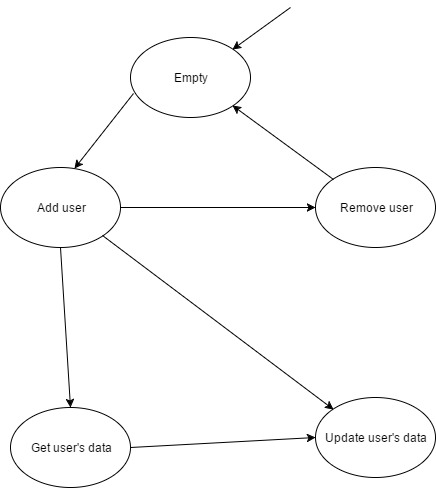
\includegraphics[width=\linewidth]{re.jpg}
  \caption{The Model Diagram of the user interface}
  \label{fig:model}
\end{figure}
\end{document}
